\%!TEX root=../document.tex

\section{Hardware-Aufbau}
\label{sec:Hardware-Aufbau}

asdfg \cite{brands11}

\begin{figure}[!htb]
	\centering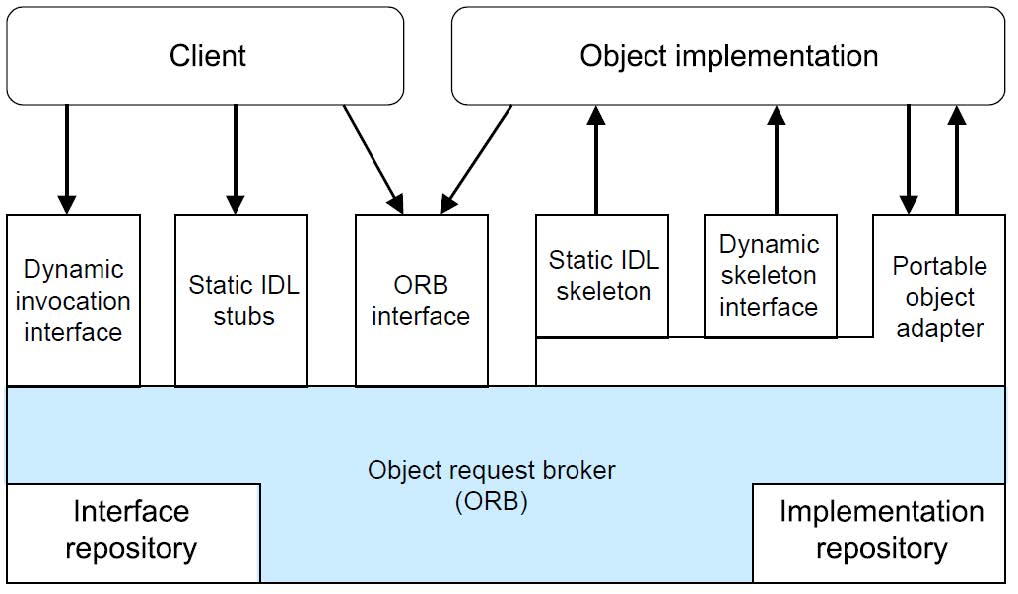
\includegraphics[width=0.8\textwidth]{images/corba.jpg}
	\caption{Ein Corba Bild}
	\label{corba}
\end{figure}

\begin{itemize}
    \item asdf
\end{itemize}


\subsection{Qubit}
\label{sec:Qubit}

\subsubsection{Schroedinger}

Schroedingers Katze ist die ber\"uhmteste Veranschaulichung eines grundlegenden Ph\"anomens der Quantenmechanik. Genaugenommen ist es ein Versuchsaufbau, anhand dessen sich verschiedene Begriffe der Quantenmechanik leicht erkl\"aren lassen. Der Versuchsaufbau sieht folgendermaßen aus:

In einer Kiste befinden sich eine Katze und eine Ampulle mit einer Giftigen Substanz. Mit einer exakten Wahrscheinlichkeit von 50\% ist die Ampulle offen und die Katze bereits tot, mit einer genau gleich großen Wahrscheinlichkeit ist aber die Ampulle immer noch verschlossen und die Katze am Leben. Da wir nur die Außenseite der Kiste sehen und sie Schall und Geruchdicht ist, k\"onnen wir nicht genau sagen, in welchem Zustand die Katze sich befindet. Es k\"onnte also behauptet werden, dass sie gleichzeitig tot und lebendig ist.
Den Umstand, dass 2 (oft gegens\"atzliche) Zust\"ande wahr sind, wird in der Quantenmechanik als Superposition bezeichnet. Eine Vorraussetzung f\"ur das erreichen einer Superposition ist die vollkommene Abschottung von der Außenwelt. 

Wenn nun die Kiste ge\"offnet wird und der Betrachter einen Blick ins innere der Kiste wirft, so erkennt er ziemlich schnell, ob die Katze tot oder lebendig ist. Einer der Beiden Zust\"ande ist durch diese sogenannte Messung verloren gegangen.

\subsubsection{Definition}

Per Definition werden die Zust\"ande eines Quantenbits in der Form \%alpha * |0> + \%beta * |1> angeschrieben.
\%alpha und \%beta werden "Amplituden" genannt, sind komplexe Zahlen und durch die Formel |\%alpha|^2 + |\%beta|^2 = 1 voneinander abh\"angig.
Anders als ein klassisches Bit, kann ein Qubit nicht gelesen, sondern muss gemessen werden, wobei die Superposition zerst\"ort wird und anhand der Amplituden (die einen Anteil darstellen) folgendermaßen berechnet werden kann, mit welcher Wahrscheinlichkeit sich das Qubit in welchem Zustand befindet: P(|0>) = |\%alpha|^2, P(|1>) = |\%beta|^2

\subsubsection{Messung}

Die Messung erfolgt je nach Ausf\"uhrung des Quantenbits, da es auf mehrere Arten realisiert werden kann. Wenn Licht eine Rolle spielt, kann die Lichtst\"arke gemessen werden, wobei diese Art von Qubits nur k\"urzer als 1 Minuten gespeichert werden kann. Kersnspinquantenbits k\"onnen durch Messung der Magnetfelder, Ionenfallen mithilfe eines Lasers ausgelesen werden. Mehr dazu befindet sich im Kapitel Anforderungen.

\subsubsection{Zust\"ande & Zustands\"anderungen}

\subsection{Register}
\label{sec:Register}

\subsubsection{Definition}
(formeln auf seite 28)

Ein Quantenregister besteht aus einer Reihe von 2 bis n Qubits und wird angeschrieben als <formel 1>
Zur Erkl\"arung ist allerdings eine Beschr\"ankung auf das Minumum von 2 Bits sinnvoll.

\subsubsection{Berechnung}

Die Berechnung des Zustands eines Quantenregisters mit 2 Bit sieht folgendermaßen aus:
<formel 2,3>

\subsubsection{Zust\"ande}

Der Zustand des Registers kann dann durch Ausmultiplizieren errechnet werden. <formel 4>

\subsubsection{begriffe "lokal" und "unit\"ar"}

\subsection{Gatter}
\label{sec:Gatter}

\subsubsection{CNOT}

CNOT bedeutet ausgesprochen "Controlled Not", was als "Kontrollierbare Negierungsschaltung" \"ubersetzt werden kann.
Ein CNOT hat 2 Eing\"ange und 2 Ausg\"ange, wobei der zweite Ausgang den invertierten Wert von 1 ausgibt wird, wenn der erste Eingang auf 1 gesetzt ist.

\subsection{Architektur}
\label{sec:Architektur}

\subsubsection{Anforderungen}

Definition von David Deutsch 1985:
Ein Quantencomputer besteht aus einer Reihe von Quantenbits,
1. die in einen Anfangszustand versetzt werden k\"onnen,
2. die Information robust speichern,
3. auf die (universelle) Quantengatter anwendbar sind und
4. die gemessen werden k\"onnen.

\subsubsection{(De)koh\"arenz}

Koh\"arenz bedeutet Zusammenh\"angend. Dekoh\"arenz ist ein Ph\"anomen der Quantenphysik, das Koh\"arenzeigenschaften von Systemen kurzzeitig außer Kraft setzt. Dekoh\"arenzeffekte treten auf, wenn ein geschlossenes System ge\"offnet wird und mit der Umwelt in Wechselwirkung treten kann, wobei die Zust\"ande beider Systeme irreversibel ver\"andert werden.
Im Beispiel mit der Katze, w\"are es eine Tote oder lebende Katze, und der Betrachter, der nun weiß, ob die Katze tot oder lebendig ist.

\subsubsection{Photonen}

Die Physiker Ludwig Mach und Ludwig Zehnder entwickelten unabh\"angig voneinander beide den selben Versuchsaufbau, der heutzutage Mach-Zender-Inferometer genannt wird. Er besteht aus 4 Spiegeln, wovon 2 halbdurchl\"assig sind, 2 Messger\"aten und einem Streifen Papier.

Wenn ein Lichtstrahl in den Aufbau geschickt wird, so wird er \"uber den ersten Spiegel, der halbdurchl\"assig ist, geteilt in eine gerade und eine um 90° abgelenkte Bahn gelenkt. Nach einem gewissen Abstand befindet sich auf jeder Bahn einer der "normalen" Spiegel, wodurch das Licht jeweils um 90° gelenkt wird und sich die beiden dann an einer Stelle kreuzen, an der der zweite halbdurchl\"assige Spiegel montiert wird. In eine Bahn wird ein Blatt Papier gehalten. Durch den halbdurchl\"assigen Spiegel kommt bei beiden Messger\"aten gleich viel Licht an. Wird das Blatt Papier entfernt, so kommt es auf einer Bahn zu konstruktiven \"uberlagerungen zwischen dem letzten Spiegel und dem Messger\"at, wodurch bei diesem kein Licht ankommt.

Wenn anstelle eines Lichtstrahles nur einzelne Photonen verwendet werden, zeigt sich der selbe Effekt, obwohl eigentlich keines der Photonen wissen kann, ob der Papierstreifen im Weg ist oder nicht. Und hier kommt wieder die Quantenphysik als Erkl\"arung zum einsatz, da ein Teilchen, wie wir schon wissen, solange es nicht beobachtet wird, in mehreren Zust\"anden gleichzeitig sein kann. Es kann sich also auf beiden Bahnen gleichzeitig bewegen, bis es gemessen wird, wodurch die Superposition zerst\"ort wird und es nur bei einem Messger\"at ankommen kann.

\subsubsection{Kernspinresonanz}

Kernspinresonanz ist der Name f\"ur einen phyiskalischen Effekt der in Form von Wechselwirkung zwischen Atomkernen und Magnetfeldern auftritt. Der Spin eines Molek\"uls kann durch Magnetfelder ausgerichtet werden, was ausgenutzt wird, um Quantenbits abzubilden und zu speichern. Durch unterschiedliche chemische Eigenschaften der Umgebung kann jedes Bit einzeln angesprochen werden. Mithilfe eines Hauptmagnetfeldes kann man die Zustande definieren, zum Beispiel als: gleiche Ausrichtung = |0>, im rechten Winkel = |1>;

\subsubsection{Ionenfallen}

Ionenfallen sind dazu da, um elektrisch geladene Molek\"ule oder Atome durch Magnetfelder an ein und der selben Position zu halten, wodurch mit einem gefangenen Ion bis zu 2 Quantenbits abgebildet werden k\"onnen. Die abst\"ande zwischen mehreren Ionen liegen im Mikrometerbereich, k\"onnen durch einen Laser einzeln adressiert werden, aber m\"ussen Temperaturm\"aßig nahe dem Absoluten gehalten werden um sich nicht gegenseitig abzustoßen.

\section{Interkommunikation}
\label{sec:Interkommunikation}


\subsection{Quantennetzwerke/Kan\"ale}
\label{sec:Quantennetzwerke/Kanale}

\subsubsection{Generelles Schema eines Telekommunikationssystems}

\subsubsection{Klassische- vs. Quanten-Kommunikationskan\"ale}

\subsubsection{Photonz\"ahlung}

Bei der Photonzälung werden zwischen 2 Standorten mit Sichtkontakt einzelne Photonen vom Sender ausgeschickt und vom Empfänger gezählt. Praktisch getestet wurde es von Harald Weinfurter im Jahr 2007 mit einer Strecke von 144 km, wofür große Teleskope verwendet werden mussten.

\subsection{Quantenteleportation}
\label{sec:Quantenteleportation}

Bei der Quantenteleportation sind 2 Atome an verschiedenen Orten durch Verschränkung verbunden, wodurch bei Anderungen an einer Seite die andere Seite gleichzeitig die selbe Änderung erfährt. Allerdings muss im Vorfeld dieses Qubit an den anderen Ort gebracht werden und zur übertragung noch eine klassische Information ausgetauscht werden, um das Qubit auf die entsprechenden Zustände projizieren zu können. Dadurch ist eine Datenübertragung auf Lichtgeschwindigkeit beschränkt und kann nicht absolut Zeitgleich erfolgen.




